\section{Ontology Overview}

\begin{figure*}
  \centering
  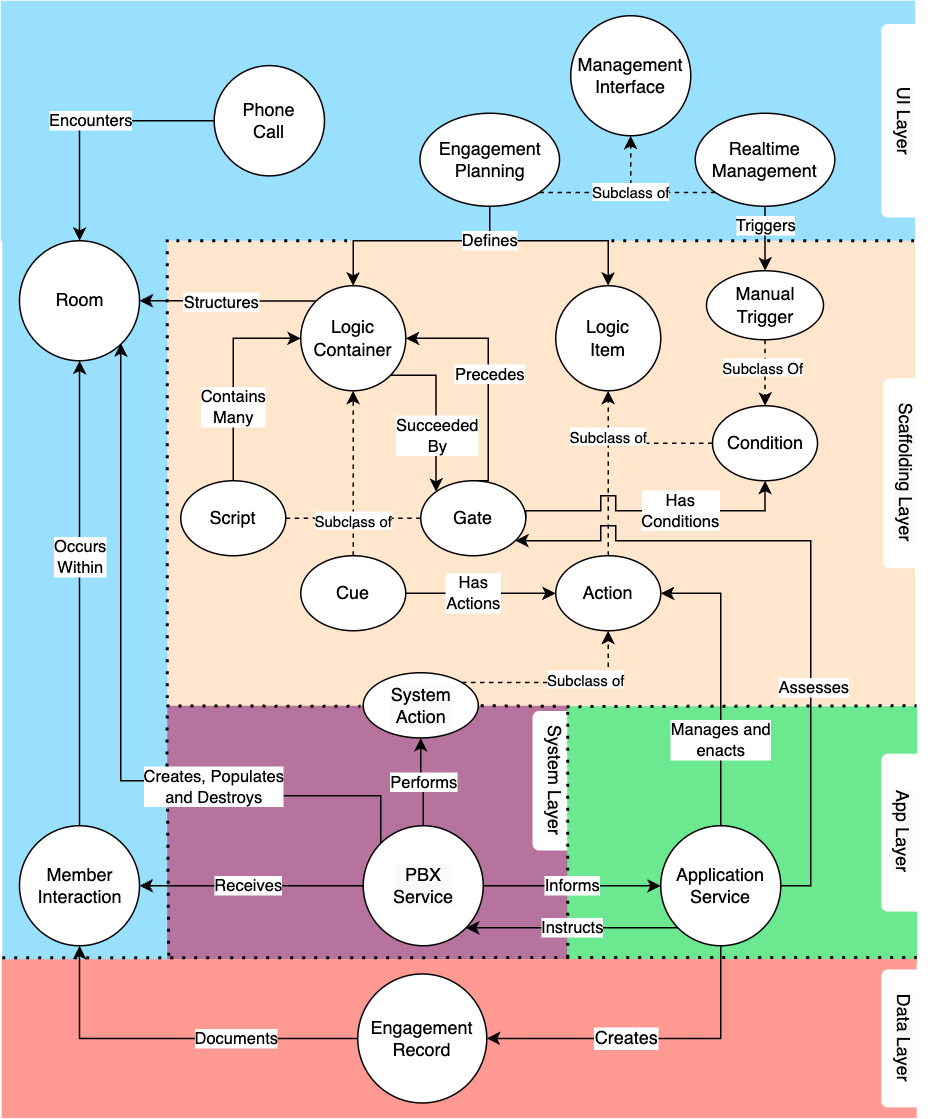
\includegraphics[width=0.8\columnwidth]{images/simplified.drawio.png}
  \caption{A visualisation of the classes and their relationships within \ONT{}, abbreviated for clarity and space. Solid arrows represent object properties (relationships). Circles depict classes whose parent classes are not shown (all are descendants from \textit{foaf} or \textit{sioc} classes). Ovals represent subclasses, connected to their parent class by dashed arrows (e.g. SystemAction is a subclass of Action).}
  \Description{A diagram giving an overview of most of the classes in \ONT{}, with labelled arrows representing relationships between classes. It is broken into five coloured layers. The first layer is blue, labelled as the "UI Layer", and contains six classes: Management interface, its subclasses Engagement Planning and Realtime Management, Phone Call, Room, and Member Interaction. Phone call encounters room. Member Interactions occur within Rooms. The next layer, the "Scaffolding Layer", is beige. It contains two parent classes: Logic container and logic item. Both are labelled as being defined by the Engagement Planning interface in the UI Layer. Logic container structures Rooms in the UI layer, and has 3 subclasses: Script, Cue and Gate. A script can contain many Logic Containers. A logic container is succeeded by a Gate, and Gates precede Logic Containers. Logic Item has two subclasses: Action and Condition. A Cue has actions, a gate has conditions. Condition has a single shown subclass, Manual Trigger, which is triggered by the Realtime Management interface in the UI Layer. Action has one shown subclass, System Action. The next layer, in green, is the "App Layer", which has one class: Application Service. Application Service assesses Gates, and manages and enacts Actions. The fourth layer is the purple "System Layer", which contains the PBX Service class. This receives Member Interactions from the UI layer, informs and receives instructions from the Application Service in the App Layer, and performs System Actions from the Scaffolding Layer. The final layer is the red "Data Layer", which contains the Engagement Record class. Engagement Records are created by the Application Service in the App Layer, and describe Member Interactions in the UI layer. }\label{fig:drawio}
\end{figure*}

Made up of relatively few classes, \ONT{} is designed to describe and structure the design space of synchronous group telephony engagement platforms, whilst still remaining abstract enough to encourage exploration, interpretation and expansion (addressing NFR2). To address NFR1, the ontology can be conceptualised as being made up of five layers of components: \textit{UI}, which describes how users and hosts interact with the system through phone calls and visual applications; \textit{Scaffolding}, which defines the components that, when combined, create the logic to orchestrates different engagement formats; \textit{System}, which describes the software (such as FreeSWITCH) by which the phone calls are initiated and manipulated; \textit{App}, which manages and enacts the Scaffolding logic and directs the System layer components;  and \textit{Data}, which refers to the data created, stored and retrieved by the App layer. 

To address NFR3, two forms of visual representation were also developed: one to communicate the relationships between the different layers of components of the ontology (Figure \ref{fig:drawio}); and the \ONT{} visual design vocabulary, which aims to support designers in designing, communicating, and understanding the technical requirements of different types of group engagements over synchronous telephony (an example is given in Figure \ref{fig:preshow}). For the sake of clarity and brevity, these diagrams exclude the base-level \textit{foaf} and \textit{sioc} axioms. The full class hierarchy is visible in Figure \ref{fig:hierarchy}. 

This section will give a detailed overview of the \ONT{} ontology, using these visuals as a communication aid.

\begin{figure}[h]
  \centering
  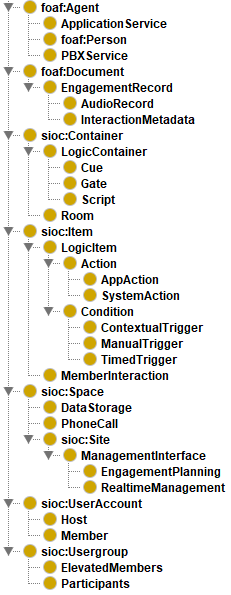
\includegraphics[width=0.25\linewidth]{images/hierarchy.png}
  \caption{Hierarchy of the classes utilised by \ONT{}, as displayed in the OWL development application Prot\'{e}g\'{e}.}
  \Description{A screenshot of the application Prot\'{e}g\'{e}, showing the list of classes within \ONT{}. Under foaf:Agent are Application Service, foaf:Person, and PBX Service. Under foaf:Document is Engagement Record, which has the subclasses Audio Record and Interaction Metadata. Under sioc:Container is Logic Container and Room. Logic Container has three subclasses: Cue, Gate and Script. Under sioc:Item is Member Interaction, Action, and Condition. Action has the subclasses App Action and System Action. Condition has the subclasses Contextual Trigger, Manual Trigger, and Timed Trigger. Under sioc:Space are Data Storage, Phone Call and sioc:Site. sioc:Site has Management Interface as a subclass, which also contains Engagement Planning and Realtime Management. sioc:UserAccount has the subclasses Host and Member. sioc:UserGroup has the subclasses Elevated Members and Participants.}
  \label{fig:hierarchy}
\end{figure}

\subsection{The UI Layer}

The UI Layer describes users and the methods by which they interact with the system---be that by a phone call or through a visual interface. Users (instances of \textit{foaf:Person}) interacting with the system are either a Host or Member (subclasses of \textit{sioc:UserAccount}). Note that while we have designed \ONT{} around interactions over standard phone calls, it's possible to apply these same concepts through other synchronous communication formats, such as WebRTC\footnote{https://webrtc.org/}---especially for Hosts, who will likely have access to an online interface.

Members are regular participants, and engage with the system through PhoneCalls (extends \textit{sioc:Space}). Through PhoneCalls, they encounter the system by populating audio spaces referred to as Rooms (extends \textit{sioc:Container}). Prior platforms only utilised a single Room, where all users were in a single conference call, but (as discussed later) multiple could be created simultaneously. MemberInteractions (extending \textit{sioc:Item}) occur inside these rooms, and could be utterances of speech or button presses. 

Hosts can access the visual ManagementInterface (extends \textit{sioc:Site}), which has two implementations depending on the state of the call: EngagementPlanning if the call is yet to start, and RealtimeManagement if it has. As an example, the Android app in \cite{Kazakos2016} is a ManagementInterface, used during the call to keep track of which participants wanted to ask questions, and mute and unmute them as needed. 

\begin{figure}[h]
  \centering
  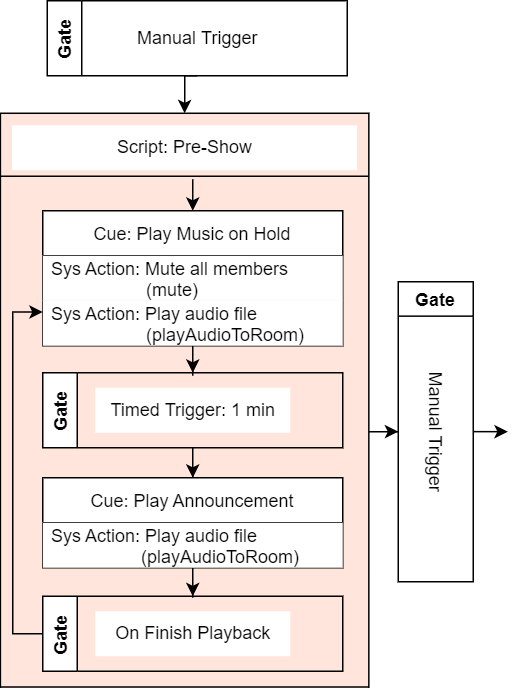
\includegraphics[width=0.4\columnwidth]{images/preshow.png}
  \caption{Using the visual design vocabulary to show how elements of the Scaffolding Layer can be configured to produce an automated pre-show routine. Here, the `Pre-Show' Script is initialised by the Host through a ManualTrigger. The Script contains four LogicContainers: two Gates and two Cues. The second Gate precedes the first Cue, forming a logic loop. This loop can be interrupted by the Host through a ManualTrigger, which would exit the Script.}~\label{fig:preshow}
  \Description{A flow chart style diagram showing how the vocabulary's components can be combined to create the logic for a pre-show routine. The first element in the flow is a Gate containing a Manual Trigger. This leads to a Script titled 'Pre-Show'. The first element inside the Script is a Cue titled 'Play Music on Hold'. It contains two Actions: 'Mute all members', which uses the mute System Action, and 'play audio file', which uses the 'play audio to room' System Action. Following this Cue is a Gate, with a Timed Trigger of one minute. Following the Gate is a second Cue, titled 'play announcement', containing one Action: 'play audio file', which uses the System Action 'play audio to room'. Following the Cue is a Gate with the Condition 'on finish playback'. The Gate then links back to the 'Play music on hold' Cue, forming a loop. The whole 'pre-show' Script is connected to another Gate with a Manual Trigger, which would interrupt the loop.}
\end{figure}

\subsection{The Scaffolding Layer}
The interplay of the components of the Scaffolding Layer creates the blueprints for different structured interactions (e.g. a Q\&A section, a breakout room session) during a call. These components are defined by the host through the EngagementPlanning interface. The permissions a participant has (e.g. if they can unmute themselves) can be controlled by assigning them to one of two subclasses of \textit{sioc:Usergroup}: ElevatedMembers or Participants (omitted from Figure \ref{fig:drawio} for space reasons). The remaining components are either LogicContainers (subclass of \textit{sioc:Container}) or LogicItems (subclass of \textit{sioc:Item}). LogicContainers contain LogicItems, and are assessed and enacted by the ApplicationService sequentially (similar to Twilio Studio). To support synchronous interactions and branching logic, multiple LogicContainers can be active at the same time (as demonstrated in Figure \ref{fig:talkshow}). A LogicContainer can be either a Script, Cue or Gate, whereas LogicItems are Actions or Conditions: 

\subsubsection{Condition (LogicItem)}

A small piece of logic relating to the call that can be evaluated to a Boolean (true or false) value. There are three main types of Conditions: TimedTriggers, which evaluate to true after a given length of time; ManualTriggers, which only become true through direct intervention by the host through the RealtimeManagement interface (e.g. the host presses a button to play an audio file); and ContextualTriggers, which can relate to particular factors within the call (e.g. `there are 10 participants present', `the audio file has finished playback'). ContextualTriggers are less formally defined in the vocabulary to support application-specific implementation.

\subsubsection{Action (LogicItem)}

An active intervention which can affect the flow of the call, managed by the ApplicationService in the Application Layer. Actions are one of two types: SystemActions and AppActions. SystemActions are performed in the System Layer as they directly interact with call audio or connections. They can be one of a limited set of interactions: \textit{dial}, \textit{hangup}, \textit{mute}, \textit{unmute}, \textit{transfer}, \textit{createRoom}, \textit{closeRoom}, \textit{playAudioToMember}, \textit{playAudioToRoom}, \textit{stopPlayback}, \textit{startRecording}, and \textit{stopRecording}. As with ContextualTriggers, AppActions are less strictly defined as they likely require per-application implementation within the ApplicationService. Examples include: `Mark participant Y as having raised their hand', `Move to the next agenda item', `Make participant X an ElevatedMember'.

The functionality required for an interaction's implementation can be identified by examining what LogicItems it uses: for example, listing the Conditions and Actions used in Figure \ref{fig:breakout} provides an answer to \textit{CQ1}.

\subsubsection{Gate (LogicContainer)}

Gates precede (and can succeed) other LogicContainers. They contain one or more Conditions connected by the logic operators AND or OR, and `unlock' once the ApplicationService in the System Layer evaluates the expression as true. For example: `The participant presses 8 AND the participant is muted'. Once the Gate is `unlocked', the LogicContainer it precedes becomes active. To support branching logic, multiple parallel Gates can be assessed simultaneously, each preceding a different LogicContainer (e.g. multiple options in an IVR menu: `\textit{press 1 to do X, press 2 to do Y}').  

\subsubsection{Cue (LogicContainer)}
Cues contain one or more Actions which are enacted when the preceding Gate is unlocked. If a succeeding Gate exists, it will start being assessed once the Cue's Actions have been initiated.

\subsubsection{Script (LogicContainer)}
Scripts contain other LogicContainers (including other Scripts) to support containerisation: allowing extended logic sequences to be initiated or interrupted by Gates. As an example, Figure \ref{fig:preshow} uses the visual design vocabulary to show a Script for a looping pre-show routine. In the routine, participants in the call are muted and music plays. After one minute, a pre-recorded announcement plays, and after it finishes the music plays again. As this Script is a LogicContainer with a succeeding Gate, the call's host can interrupt this loop at any time to start the show. If no loop is present, the final LogicContainer will exit the script upon completion (as seen in Figures \ref{fig:breakout} and \ref{fig:roundrobin}).

As will be demonstrated in Section \ref{section:scenarios}, through such combinations of Conditions, Gates, Actions, Cues, and Scripts, we can use \ONT{} to describe complex interactions.

\subsection{The Application Layer}

The Application Layer contains the ApplicationService: a software application (e.g. built using PHP, as in  \cite{Kazakos2016}) which puts the Scaffolding Layer into practice, assessing currently active Gates and managing any resulting Actions. It enacts all except SystemActions, which it instructs the System Layer (described below) to perform. The ApplicationService is a \textit{foaf:Agent}, as it is capable of programmatically taking independent action in response to changes in state.

\subsection{The System Layer}

The System Layer features the PBXService (also a \textit{foaf:Agent}): the key server-side component common to previous synchronous telephony platforms \cite{Kazakos2016, Talhouk2017, Yadav2017}. PBXService is an application capable of programmatically initiating and managing voice connections (e.g. via Voice Over IP, or the Public Switched Telephone Network) and creating, populating and destroying Rooms. FreeSWITCH is an example of a PBXService, and was used by Kazakos et al. in their project \cite{Kazakos2016}. Another popular example is Asterisk \footnote{https://www.asterisk.org/}. The PBXService enacts SystemActions and informs the ApplicationService of any changes in the call state, such as instances of MemberInteractions (e.g. buttons presses, vocal utterances, disconnections).

\subsection{The Data Layer}

The Data Layer concerns the storage of data, either for use within a call (e.g. playback of existing audio) or archiving. EngagementRecords (subclass of \textit{foaf:Document}) can either be AudioRecords or InteractionMetadata, and are created by the ApplicationService to document MemberInteractions. As an example of how these could be used, the process described in Figure \ref{fig:talkshow} could keep records of which Members raised their hands and which were unmuted---data which could be queried to answer \textit{CQ2}.